\section{Evaluation: eval mode, metrics and results}
\label{sec:eval}

\subsection{What changes in eval mode}
\label{sec:evalbn}

\begin{idea}[BN collapses to a per-channel affine map]
With the running statistics frozen, BN no longer depends on the batch:
\[
  y = \gamma_c\frac{x-r_{\mu,c}}{\sqrt{r_{\sigma^2,c}+\varepsilon}}+\beta_c
    = a_c\,x + b_c,\qquad a_c=\frac{\gamma_c}{\sqrt{r_{\sigma^2,c}+\varepsilon}},\quad b_c=\beta_c-a_c\,r_{\mu,c}.
\]
Because the preceding conv is linear, the BN could even be \emph{folded} into it: $\mathcal W'[o]=a_o\mathcal W[o]$, bias $b_o$. The repo does not fold. Eval-mode predictions are deterministic and independent of what else is in the batch, so a batch of 1 in the service behaves exactly like a batch of 128 in the evaluation.
\end{idea}

\begin{repo}[\texttt{evaluate()} and \texttt{predict()}]
Both call \code{model.eval()} and run inside \code{torch.no\_grad()}, so no graph is stored and the BN buffers are not touched. \code{evaluate} returns the example-weighted mean loss and the accuracy. \code{predict} returns \code{softmax(logits, dim=1)} for every test image as a NumPy array \shp{10000,10} plus the labels \shp{10000}. \file{eval\_test.py} saves both to \file{artifacts/preds/<name>.npz}, and every metric below is computed from that file. ResNet has no dropout, so BN is the only layer whose behaviour differs between the two modes.
\end{repo}

\subsection{Confusion matrix}

\begin{idea}
$C\in\mathbb N^{10\times10}$ with $C[t,p]=\#\{\text{test images of true class }t\text{ predicted as }p\}$. Rows sum to the class sizes (1{,}000 each), and the trace counts the correct predictions. Accuracy $=\operatorname{tr}(C)/\sum C$.
\end{idea}

\begin{repo}[the final ResNet-20 on the 10{,}000 test images]
\begin{center}
\scriptsize
\setlength{\tabcolsep}{4.5pt}
\begin{tabular}{@{}r|cccccccccc|r@{}}
true $\backslash$ pred & plane & car & bird & \textbf{cat} & deer & \textbf{dog} & frog & horse & ship & truck & recall\\
\midrule
plane & \textbf{923} & 4 & 23 & 10 & 5 & 0 & 3 & 1 & 19 & 12 & 0.923\\
car & 7 & \textbf{966} & 0 & 0 & 0 & 0 & 0 & 0 & 2 & 25 & 0.966\\
bird & 20 & 0 & \textbf{884} & 23 & 24 & 18 & 20 & 5 & 4 & 2 & 0.884\\
\textbf{cat} & 11 & 0 & 23 & \textbf{822} & 25 & \cellcolor{warn!25}76 & 21 & 11 & 4 & 7 & 0.822\\
deer & 2 & 0 & 23 & 14 & \textbf{927} & 12 & 6 & 14 & 0 & 2 & 0.927\\
\textbf{dog} & 4 & 0 & 14 & \cellcolor{warn!25}85 & 17 & \textbf{865} & 5 & 8 & 2 & 0 & 0.865\\
frog & 2 & 1 & 25 & 18 & 8 & 4 & \textbf{939} & 1 & 1 & 1 & 0.939\\
horse & 5 & 0 & 5 & 16 & 21 & 26 & 2 & \textbf{922} & 2 & 1 & 0.922\\
ship & 23 & 4 & 4 & 3 & 0 & 0 & 0 & 0 & \textbf{956} & 10 & 0.956\\
truck & 10 & 22 & 1 & 3 & 0 & 1 & 2 & 1 & 6 & \textbf{954} & 0.954\\
\midrule
precision & .917 & .969 & .882 & .827 & .903 & .863 & .941 & .957 & .960 & .941 & \\
\end{tabular}
\end{center}
Trace $=9{,}158$, so accuracy $=91.58\%$ and test error $=\mathbf{8.42\%}$. The two shaded cells, cat$\to$dog (76) and dog$\to$cat (85), are the largest off-diagonal entries, together 161 of the 842 errors. The other classic CIFAR confusions are visible too: car$\leftrightarrow$truck (25 + 22) and plane$\leftrightarrow$ship (19 + 23).
\end{repo}

\subsection{Precision, recall, F1}

\begin{idea}[row and column sums of $C$]
For class $k$: $TP_k=C[k,k]$, $FP_k=\sum_tC[t,k]-TP_k$ (column), $FN_k=\sum_pC[k,p]-TP_k$ (row). Then
\[
  \text{precision}_k=\frac{TP_k}{TP_k+FP_k},\qquad \text{recall}_k=\frac{TP_k}{TP_k+FN_k},\qquad F1_k=\frac{2\,\text{prec}_k\,\text{rec}_k}{\text{prec}_k+\text{rec}_k}.
\]
Worked for cat: $TP=822$, the cat column sums to $994$, so precision $=822/994=0.827$; the cat row sums to $1000$, so recall $=0.822$; $F1=2(0.827)(0.822)/(1.649)=0.824$.
\end{idea}

\begin{repo}
\code{per\_class\_metrics(C)} implements exactly this with \code{np.diag}, \code{C.sum(axis=0)} (columns) and \code{C.sum(axis=1)} (rows), and uses \code{np.divide(..., where=...)} to return 0 instead of dividing by zero for a class that is never predicted. The mean F1 is $0.9158$. It equals the accuracy here only because every class has exactly 1{,}000 test images and precision $\approx$ recall per class.
\end{repo}

\subsection{Calibration and expected calibration error}
\label{sec:calib}

\begin{idea}[does a 0.9 confidence mean 90\% correct?]
For each test image let $\text{conf}_i=\max_k s_{ik}$ and $\text{correct}_i=[\hat y_i=y_i]$. Split $(0,1]$ into $B=15$ equal bins $I_b=(\tfrac{b-1}{15},\tfrac{b}{15}]$ and let $\mathcal B_b=\{i:\text{conf}_i\in I_b\}$. Then
\[
  \text{ECE} = \sum_{b=1}^{15}\frac{|\mathcal B_b|}{n}\,\Big|\underbrace{\tfrac{1}{|\mathcal B_b|}\textstyle\sum_{i\in\mathcal B_b}\text{correct}_i}_{\text{acc}(b)} - \underbrace{\tfrac{1}{|\mathcal B_b|}\textstyle\sum_{i\in\mathcal B_b}\text{conf}_i}_{\text{conf}(b)}\Big| .
\]
A perfectly calibrated model has acc$(b)=$conf$(b)$ in every bin and ECE $=0$.
\end{idea}

\begin{repo}[\texttt{calibration(probs, labels, n\_bins=15)}]
\begin{center}
\scriptsize
\setlength{\tabcolsep}{3.2pt}
\begin{tabular}{@{}lrrrrrrrrrrr@{}}
\toprule
bin upper edge & $\le\!\frac{4}{15}$ & $\frac{5}{15}$ & $\frac{6}{15}$ & $\frac{7}{15}$ & $\frac{8}{15}$ & $\frac{9}{15}$ & $\frac{10}{15}$ & $\frac{11}{15}$ & $\frac{12}{15}$ & $\frac{13}{15}$ & $\frac{14}{15}$\;/\;1\\
\midrule
$|\mathcal B_b|$ & 0 & 3 & 15 & 26 & 81 & 126 & 111 & 123 & 145 & 208 & 308\;/\;\textbf{8854}\\
acc$(b)$ & -- & .333 & .400 & .154 & .469 & .468 & .523 & .520 & .524 & .625 & .640\;/\;.963\\
conf$(b)$ & -- & .316 & .375 & .432 & .508 & .568 & .634 & .699 & .768 & .835 & .903\;/\;.997\\
\bottomrule
\end{tabular}
\end{center}
ECE $=0.0521$. The mean confidence is $0.968$ against an accuracy of $0.916$. In almost every bin confidence exceeds accuracy, so the model is \textbf{overconfident}. 88.5\% of all predictions land in the top bin, where the model claims 99.7\% and is right 96.3\% of the time. That single bin contributes $0.885\times0.034=0.030$ of the ECE. Bins are half-open $(lo,hi]$ via \code{(conf > lo) \& (conf <= hi)}. A confidence of exactly 0 would be missed, but it is impossible here since $\max_k s_k\ge0.1$.
\end{repo}

\begin{center}
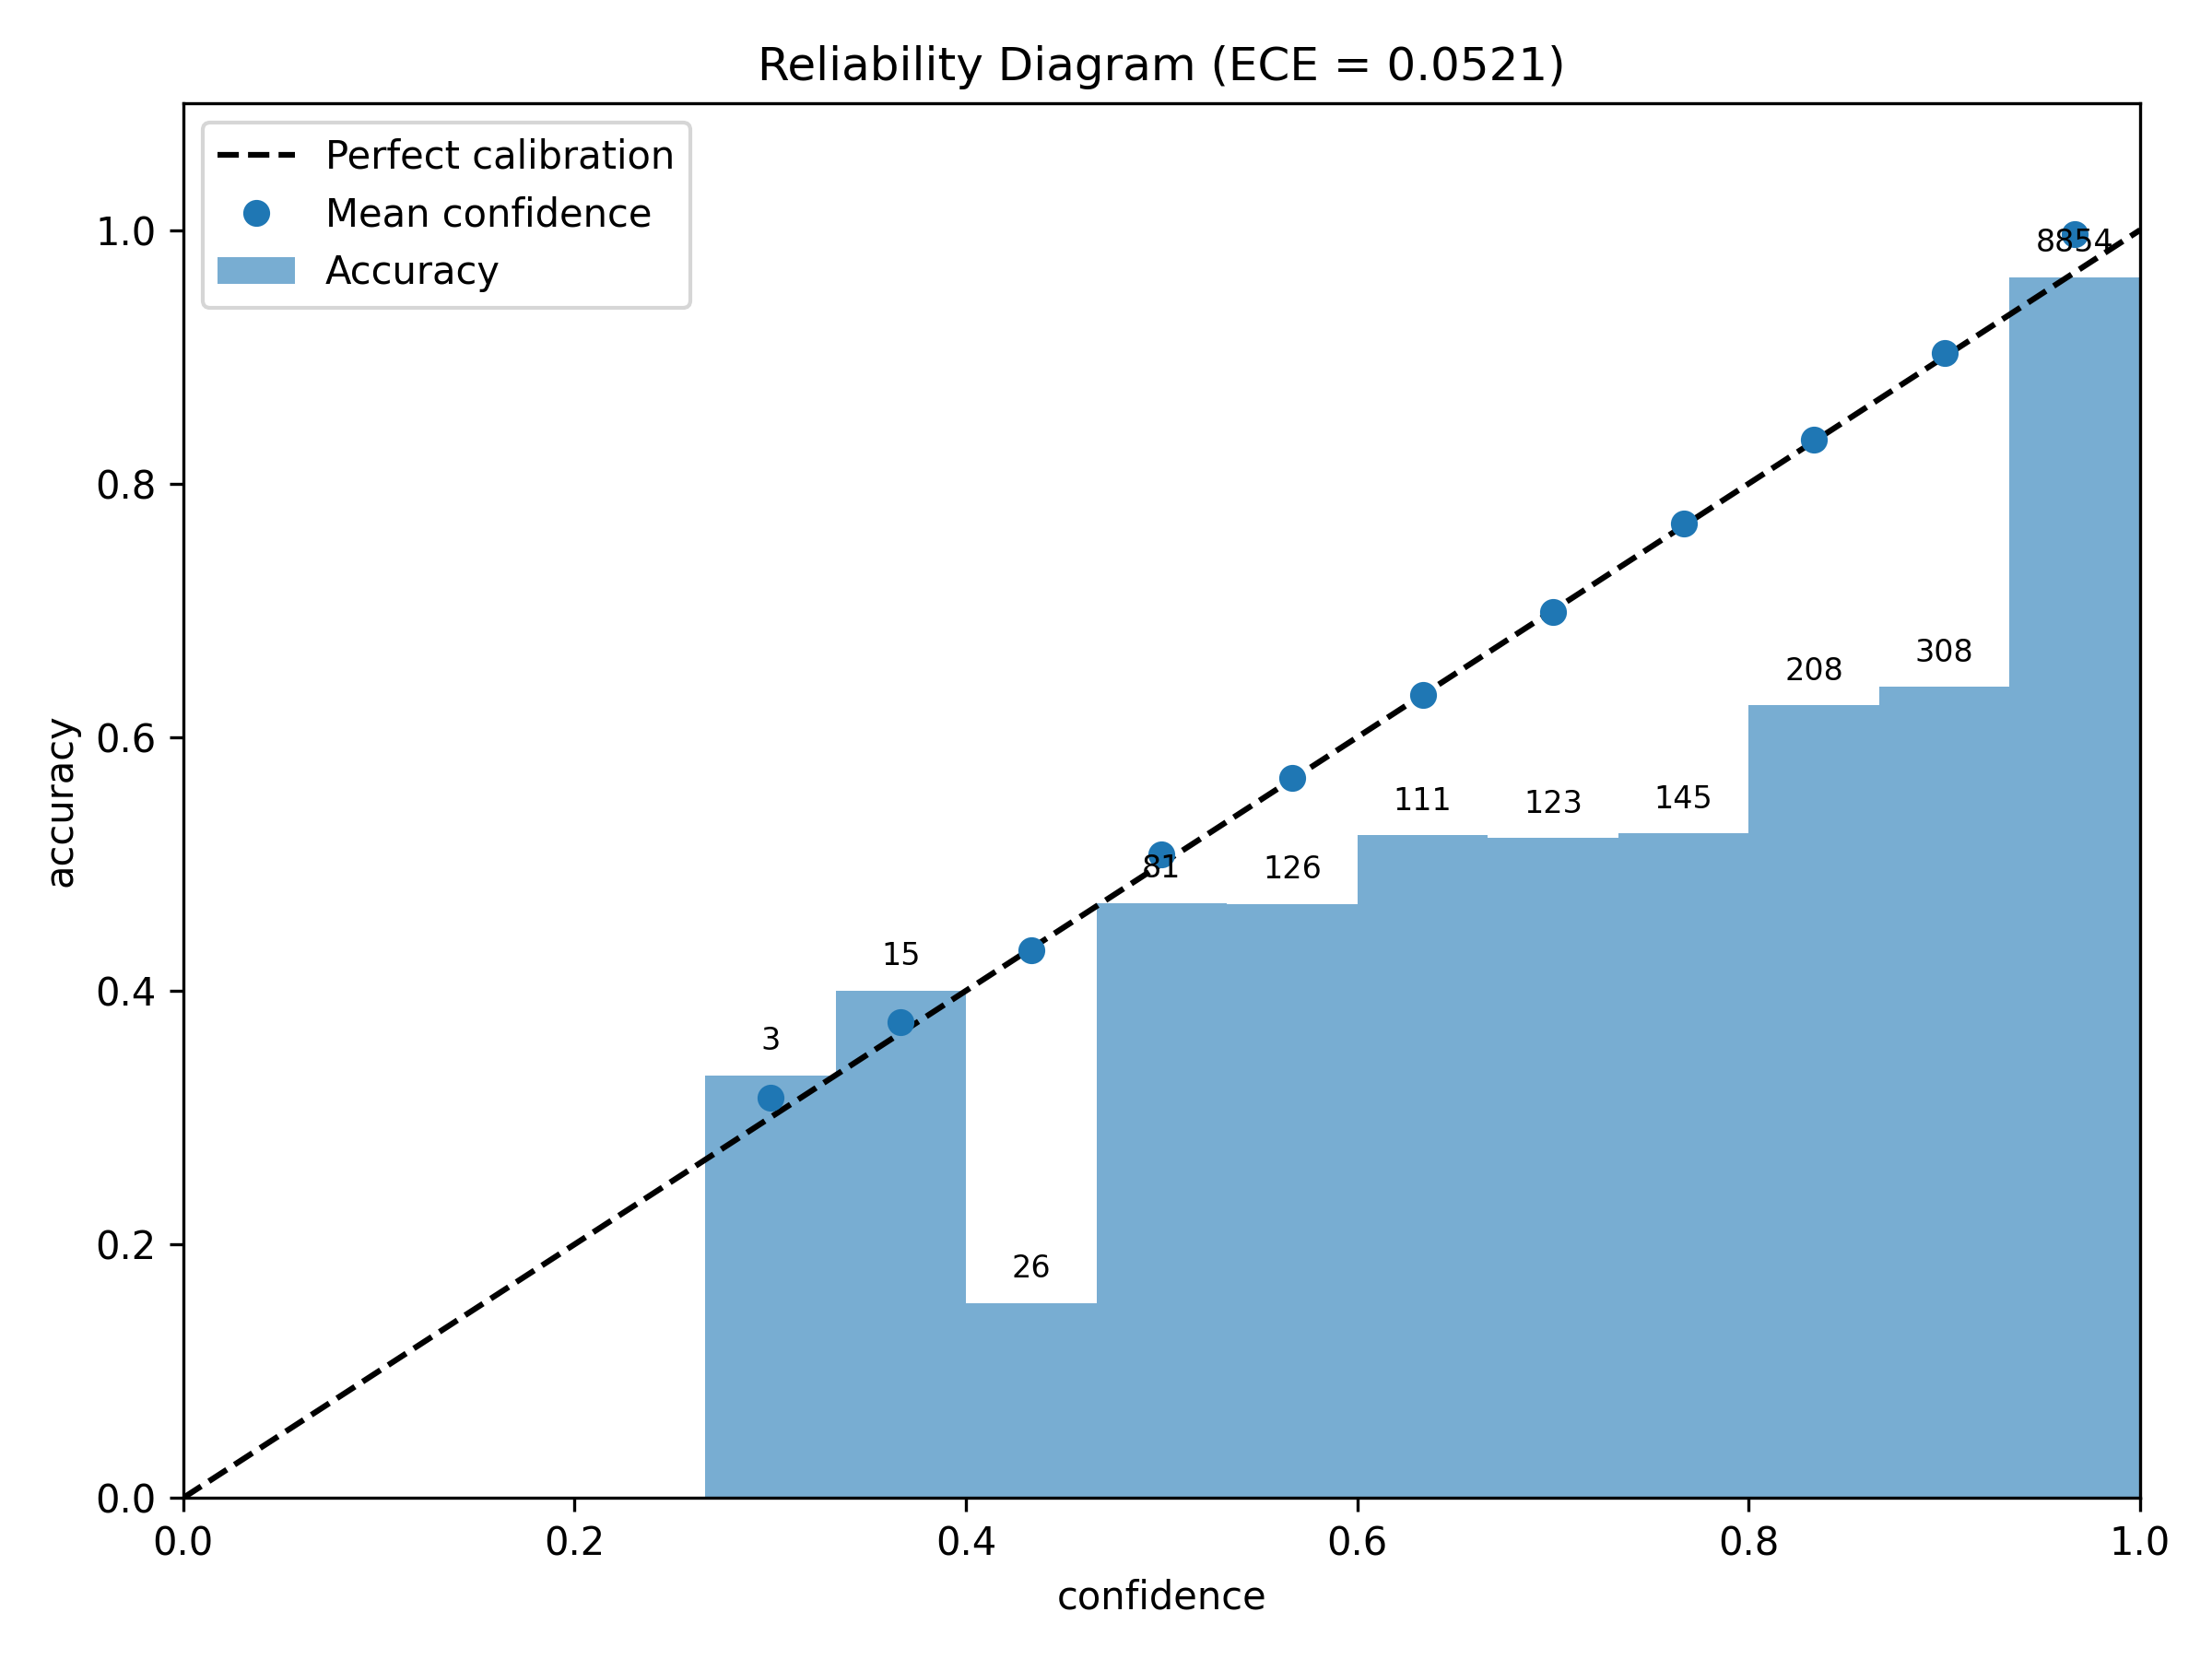
\includegraphics[width=0.47\linewidth]{../figures/reliability.png}\hfill
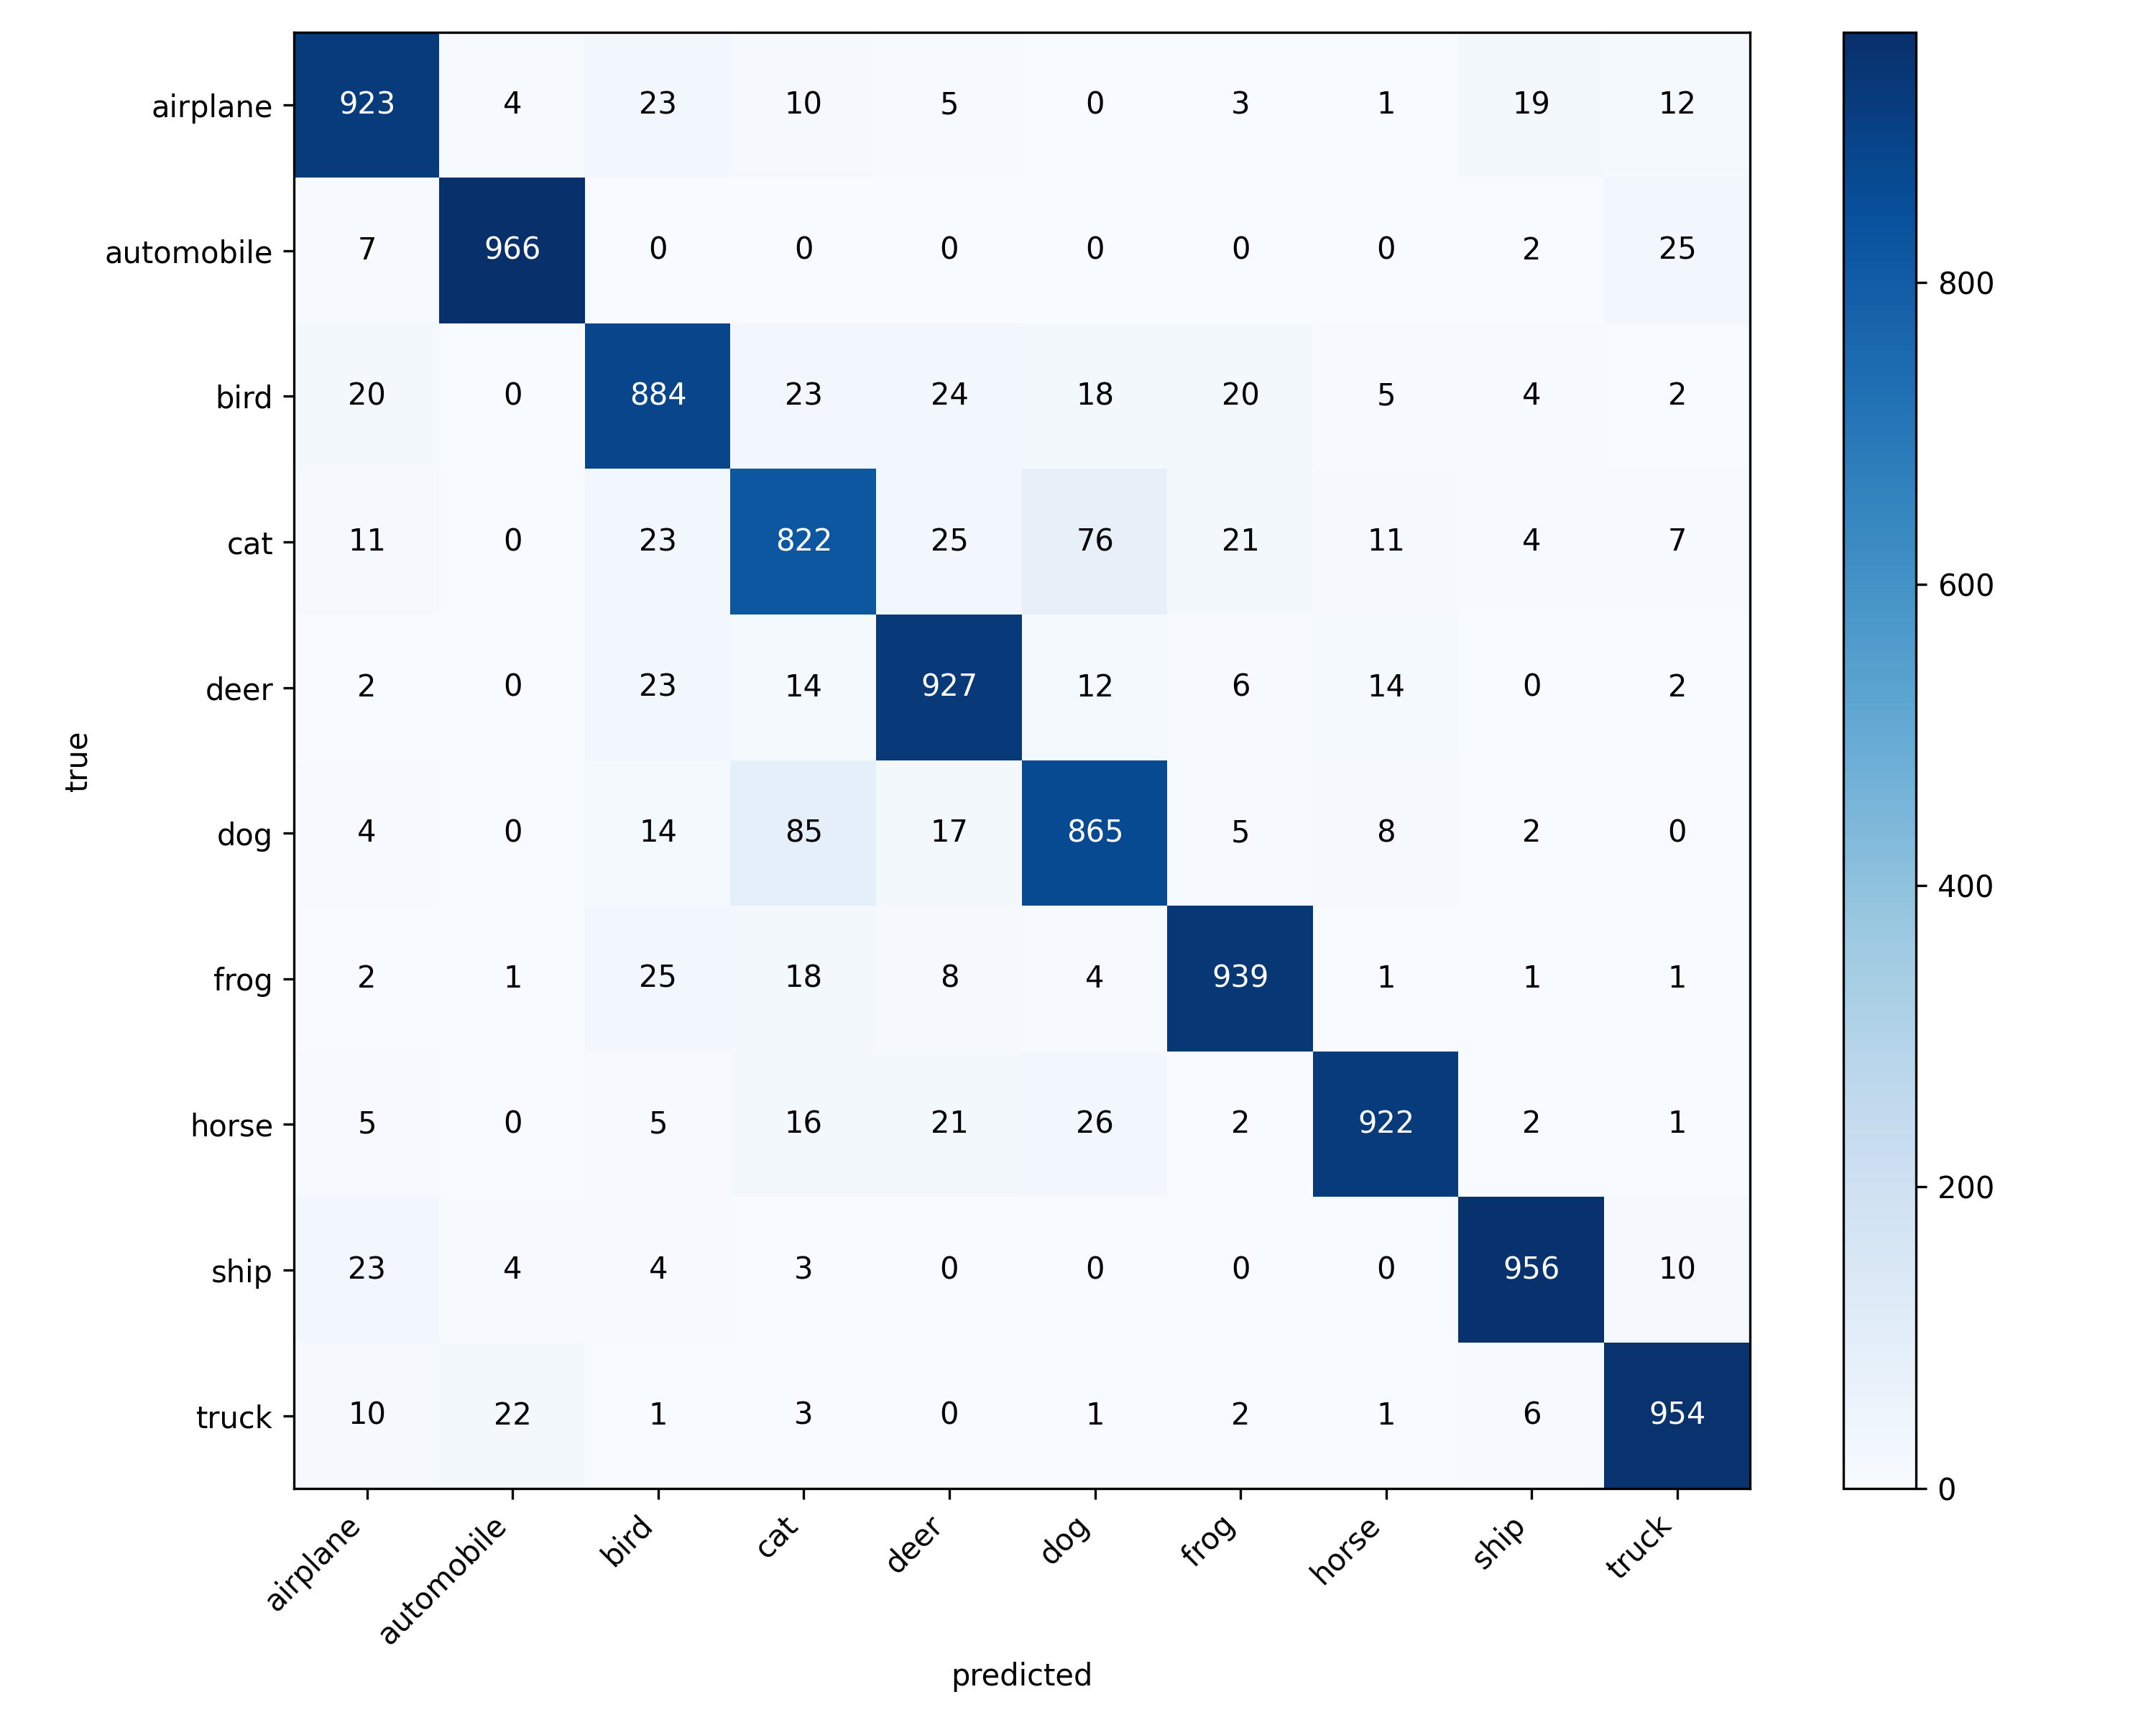
\includegraphics[width=0.47\linewidth]{../figures/confusion.png}
\end{center}

\begin{center}
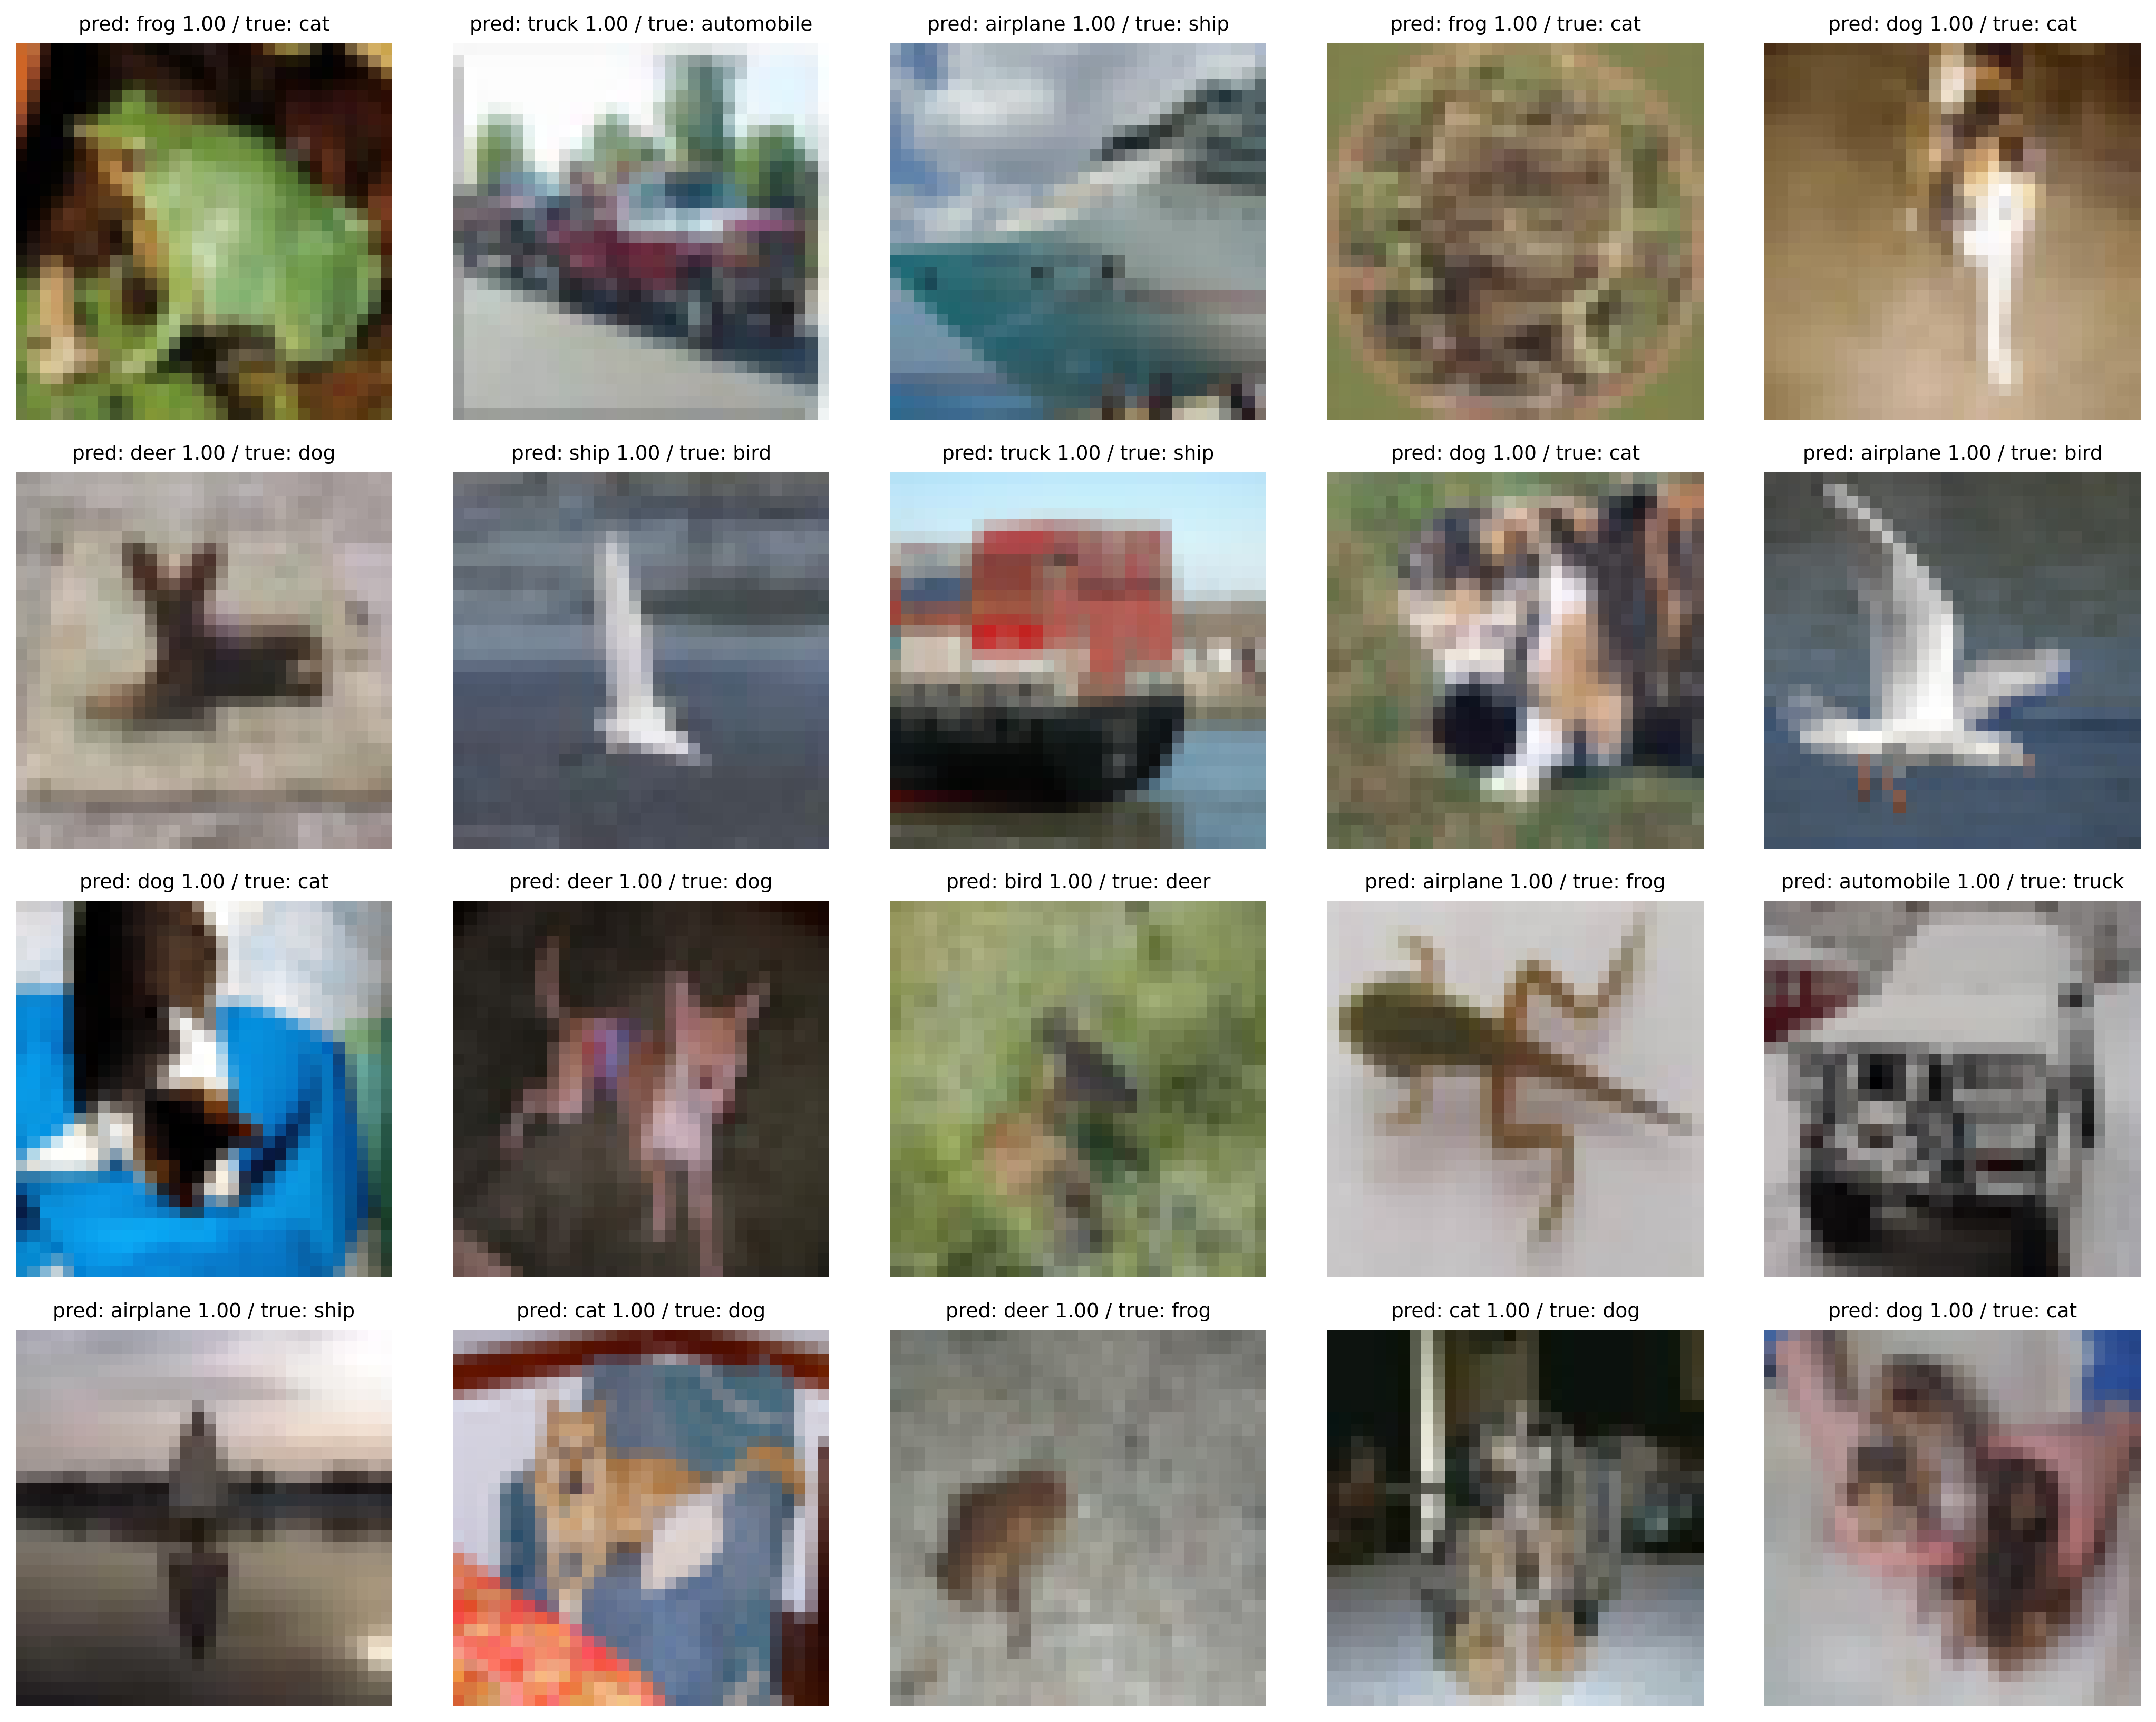
\includegraphics[width=0.85\linewidth]{../figures/confident_errors.png}

\small The 20 most confident wrong predictions (\file{docs/figures/confident\_errors.png}). Six are cat$\leftrightarrow$dog swaps, and the first is plausibly a label error in the dataset.
\end{center}

\subsection{Headline result}

\begin{repo}
\begin{center}
\begin{tabular}{@{}lrr@{}}
\toprule
model & test error, this repo & test error, paper\\
\midrule
ResNet-20 (trained on 50k, 64k iterations) & 8.42\% & 8.75\%\\
\bottomrule
\end{tabular}
\end{center}
Both are single runs. The paper's 5-run spread for ResNet-110 is $\pm0.16$ points, so a 0.33-point gap is ``matches the paper'', not ``beats it''. The test set was used once, after all choices had been made on the 45k/5k split.
\end{repo}

\subsection{Depth ablation: plain vs.\ residual}
\label{sec:ablation}

\begin{repo}[same recipe, 45k training images, seed 0]
\begin{center}
\begin{tabular}{@{}lrlrrr@{}}
\toprule
run & depth & type & train error & val error & test error\\
\midrule
ResNet-20 & 20 & residual & 0.52\% & 8.26\% & 9.29\%\\
plain-20 & 20 & plain & 0.88\% & 9.22\% & 9.77\%\\
ResNet-56 & 56 & residual & 0.08\% & 6.88\% & \textbf{7.92\%}\\
plain-56 & 56 & plain & \textbf{3.72\%} & 12.00\% & 12.94\%\\
\bottomrule
\end{tabular}
\end{center}
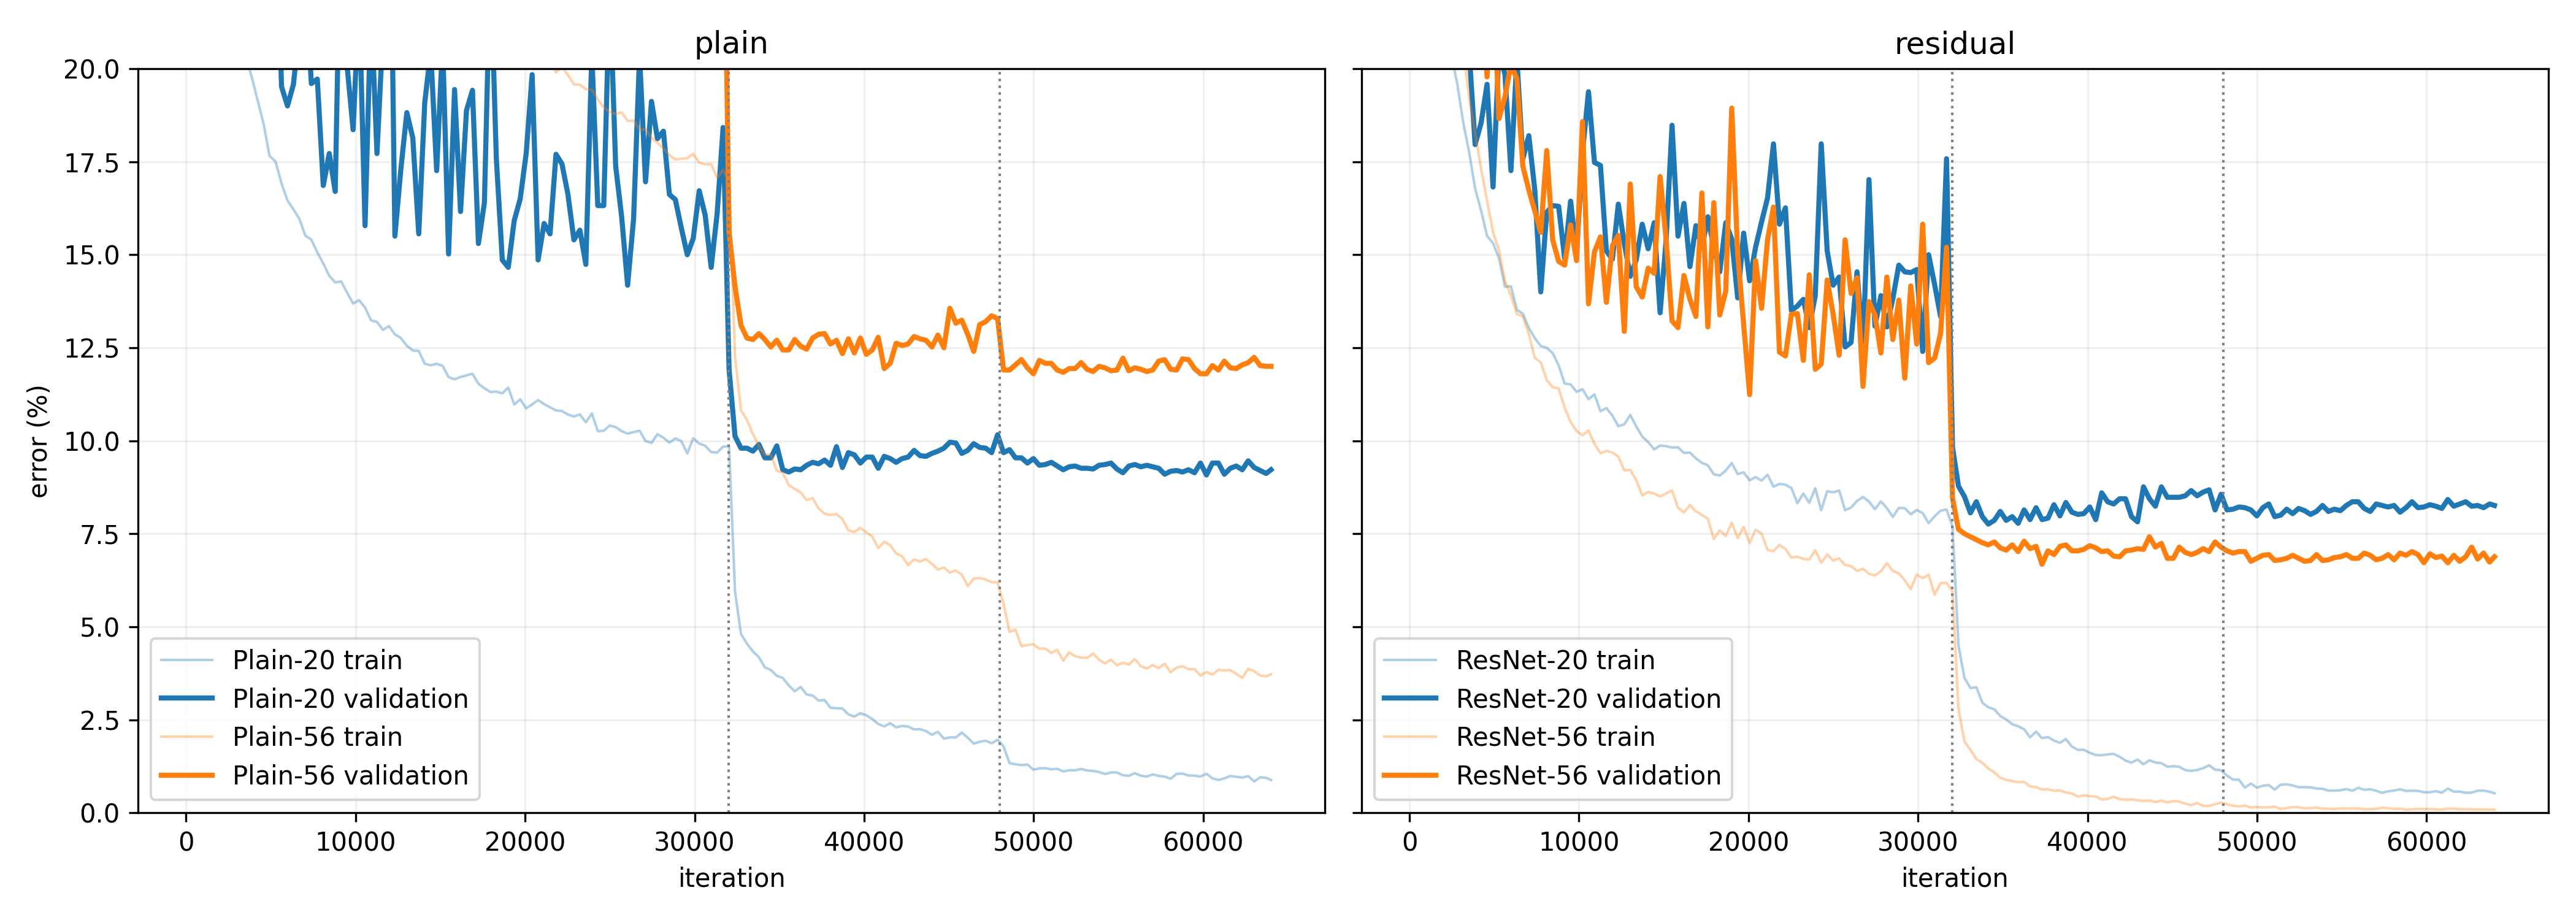
\includegraphics[width=\linewidth]{../figures/curves.png}
Going from 20 to 56 layers makes the plain network \emph{worse} (test $9.77\to12.94\%$), and its \emph{training} error rises too ($0.88\to3.72\%$). The deeper plain net is not overfitting. It fails to optimise, which is the degradation problem the paper set out to solve. The residual network improves with depth ($9.29\to7.92\%$). The two pairs have identical parameters and FLOPs (853{,}018 for both 56-layer nets), so the shortcut connection is the only difference. ResNet-56 takes 5{,}171\,s ($\approx86$ min) vs.\ 2{,}238\,s for ResNet-20 on the same GPU.
\end{repo}
